% !TEX root = ../ausarbeitung.tex

\chapter{Stand der Forschung}

Die Motivation der Arbeit beruht auf Erkenntnissen zu Behandlungsformen für Lese- Rechtschreibschwäche (LRS). Es wurde untersucht, wie gut der Prozess des Erzeugens von Übungstexten automatisiert werden kann. Hierfür war das Ziel bei der Entwicklung der Applikation eine möglichst gute User Experience zu bieten. Die Zielgruppe, bestehend aus LerntherapeutInnen, Lehrkräften und Eltern betroffener Kinder, soll das Programm möglichst intuitiv bedienen können.\\
Im Folgenden werden daher erst die Grundlagen zu LRS erklärt und digitale Ansätze zur Erstellung von Übungstexten, z.B. auch ähnliche, bereits vorhandene Software beschrieben. Danach werden die technischen Grundlagen und computerlinguistische Begriffe erklärt, die in der Entwicklung der Applikation relevant waren.

\section{Lese- Rechtschreibschwäche}

Ein Ausgangspunkt zur Feststellung von LRS bietet die Lesekompetenz. Eine Definition aus der PISA Studie untergliedert die Lesekompetenz in die vier Teilbereiche \textit{Kognitive Grundfähigkeit}, \textit{Dekodierfähigkeit}, \textit{Lernstrategiewissen} und \textit{Leseinteresse}\cite{Schulte-Koerne2014}.\\
Der Teilbereich, zu dessen Verbesserung diese Arbeit einen Beitrag leisten kann ist die Dekodierfähigkeit. Diese stellt die Kompetenz dar, die Bedeutung von Wörtern, Sätzen und Texten zu erfassen und zu verstehen. Die Unterteilung in die drei Elemente Wort, Satz und Text stellt eine Dekodierungsfähigkeit auf verschiedenen Ebenen dar, die sich gegenseitig bedingen. Das Wort ist hier die Basisebene. So kann ein Text nur verstanden werden, wenn die Bedeutung der einzelnen Sätze erfasst wurde und diese wird wiederum nur erkannt, wenn eine ausreichende Dekodierfähigkeit für Wörter vorhanden ist. Somit ist eine Voraussetzung für die Verbesserung des Textverständnis, dass das Erkennen des Basiselements Wort beherrscht wird.

\subsection{Dekodierung des Wortbildes}
\label{sec:dekodierung}

Es ist bekannt, dass Kinder in der Entwicklung des Lesens und Schreibens verschiedene Phasen durchlaufen\cite{Steinbrink2014}. So gibt es in jedem Fall eine alphabetische und eine orthographische Phase. Beim Lesen wird in der alphabetischen Phase ein Wort Buchstabe für Buchstabe dekodiert, \textit{Grapheme} (die kleinste Einheit in der Schriftsprache, in der deutschen Sprache Buchstaben) werden einzeln in \textit{Phoneme} (Laute, die kleinste Einheit der gesprochenen Sprache) umgewandelt, was aber bei nicht lautgetreuen Wörtern (Wörter, in denen sich nicht alle Grapheme korrekt in die zugehörigen Phoneme übersetzen lassen) nicht gelingt.\\
Daher wird später in der orthographischen Phase eine Strategie benutzt, die sich an größeren Bestandteilen orientiert. Wörter oder Wortteile werden hier aus dem Langzeitgedächtnis abgerufen, was bei richtig gelernten Silben und Wörtern zu korrekter Aussprache und Schreibung führt.\\
Einige schulische Ansätze wie das \textit{ABC der Tiere}\cite{mildenberger2013} oder die \textit{Freiburger Rechtschreibschule (FRESCH)}\cite{Fresch2016} fördern das orthographische Lernen mit einer gezielten Hervorhebung von Silben. Hier sind z.B. Fördermaterialien erhältlich, die Silben farblich hervorheben um Lernerfolge beim Schrifterwerb zu erzielen.\\

Weiterführende Arbeiten legen auch nahe, dass der Sprachrhythmus und die Silbenbetonung eine zentrale Rolle, sowohl beim Lesen, als auch beim Schreiben spielt. Ein Wort hat in der deutschen Sprache eine oder mehrere Betonungen. Betonte Silben werden, im Gegensatz zu den unbetonten Silben, lauter und länger gesprochen. In der Dissertation von Brandelik\cite{Brandelik2014} wurde gezeigt, dass sprachrhythmische Fähigkeiten, wie das Identifizieren von Betonungen einen Einfluss auf die Lese- und Rechtschreibleistung hat. An diese Ergebnisse angelehnt trainiert z.B. die Prosodiya App\cite{Holz2017} für mobile Geräte bei LRS Kindern das Bewusstsein für linguistische Eigenschaften im Zusammenhang mit der Silbenbetonung.\\
In einer Studie von Rello\cite{Rello:2017:PMR:3057333.3057414} wurde zudem herausgefunden, dass die Art der Präsentation von Text ein starken Einfluss auf die Lesbarkeit für Menschen mit LRS hat. Es wurde gezeigt, dass Parameter wie verschiedene Fonts, Schriftgröße, Farbkombinationen und Hintergrundfarbe, sowie die Abstände zwischen Zeilen oder einzelnen Zeichen eine wesentliche Rolle für die Lesegeschwindigkeit spielen.

\subsection{Digitale Ansätze}
\label{sec:lrs-digital}

In der Recherche für die Entwicklung der Webapplikation wurde auch untersucht, welche ähnlichen Software-basierten Lösungen es schon gibt. Das im vorherigen Abschnitt erwähnte \textit{ABC der Tiere} liefert auch einen \textit{Silben-Generator}\cite{ABCSilbengenerator2018}. Dieser ist allerdings nur als Windows Programm erhältlich und die Möglichkeiten des Programms sind sehr begrenzt. So gibt es z.B. kein Textfeld, in das man selbst Text eingeben kann, es ist nur das Laden von Textdateien möglich. Es gibt hier auch nur wenige Einstellungen, so kann man zwar Silbenfarben und Zeilenabstand anpassen, nicht jedoch den Abstand zwischen Wörtern oder Silben. Einstellungen lassen sich auch nur global ändern und nicht, z.B. bezogen auf einzelne Texte speichern.

\begin{figure}[h!]
	\centering
	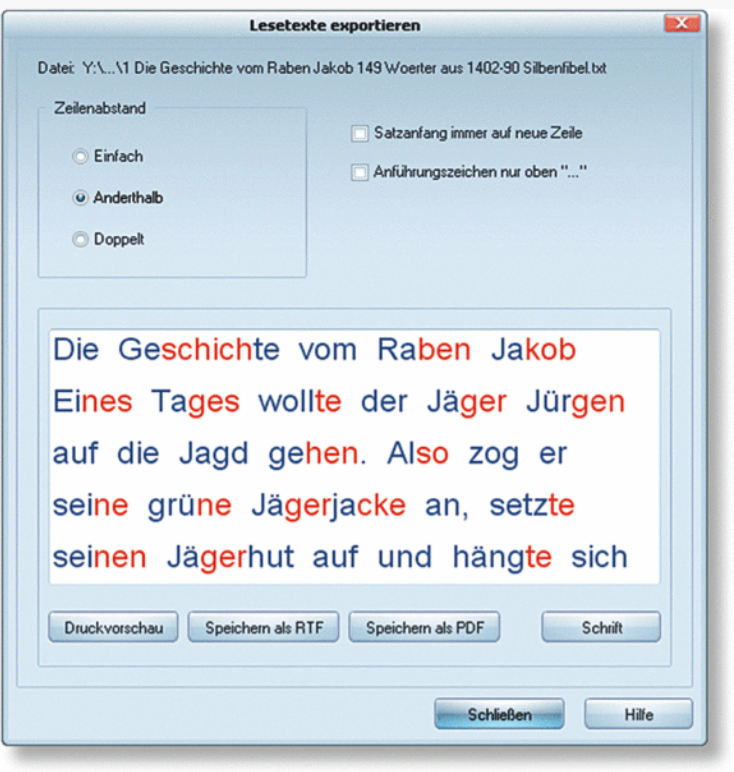
\includegraphics[width=.5\linewidth]{figures/ABCsilbengenerator}
	\caption{Bildschirmfoto des Silbengenerators auf der Internetseite von \textit{ABC der Tiere}\cite{ABCSilbengenerator2018}}
	\label{fig:ABCsilbengenerator}
\end{figure}

Ein weiteres zu erwähnendes Tool ist die \textit{Celeco Druckstation}\cite{celeco2018}. Auch hier können eigene Texte entweder mit farblich markierten Silben oder Silbenbögen gedruckt werden. Das Programm ist zusammen mit der \textit{Celeco} Software (LRS Therapie und Leseübungen) erhältlich, welche für Windows verfügbar ist.

Um die Vorteile durch silben- und betonungsorientiertes Lernen auszunutzen ist man oft auf Materialien von Verlagen oder eine aufwendige manuelle Erstellung von Texten angewiesen. Dies bekräftigt die Motivation eine neue Lösung zu entwickeln, um eigenes Übungsmaterial erstellen zu können, was zudem flexibel gestaltbar und z.B. auf bestimmte Schüler anpassbar ist.

\section{Technischer Hintergrund}

Um das Ziel einer automatischen Analyse und Annotation beliebiger Texte zu realisieren, wurden vor Allem die folgenden zwei Schritte untersucht:
\begin{enumerate}
	\item Linguistische Analyse (Zerlegung des Texts in Wörter)
	\item Bestimmung von Silbentrennung und Betonungsmuster
\end{enumerate}

\subsection{Linguistische Analyse}
Da die von der Applikation zu verarbeitende Eingabe ein Text ist, also eine Folge von alphanumerischen Zeichen, sowie Leerraumzeichen und Interpunktionen, muss diese Eingabe zunächst korrekt in Wörter zerteilt werden. Dieser Schritt wird \textbf{Tokenisierung} genannt. Zusätzlich werden auch von einem \textbf{Tagger} jedem Wort weitere Informationen, wie z.B. die Wortart (\textit{Part-of-Speech-/POS-Tagger}) hinzugefügt. Diese werden üblicherweise mithilfe eines entsprechenden Lexikons nachgeschlagen\cite{Carstensen2004}. Der für dieses Projekt verwendete Parser wird in Abschnitt \ref{sec:spacy} näher beschrieben. Beim Parsen des Texts können folgende wichtige Informationen extrahiert werden:

\begin{itemize}
	\item \textbf{Textstruktur}: Zerlegung des Texts in Tokens, dadurch wird bestimmt, ob es sich bei den Zeichenfolgen um Wörter oder andere Strukturen wie Leerraum oder Interpunktionen handelt.
	
	\item \textbf{Wortart}: Die Werte der Wortart- (\textit{Part-of-Speech-}) Tags geben an um was für ein Wort es sich handelt (mit dem \textit{spacy} Parser z.B. \textit{NOM} für Nomen, \textit{PROPN} für Eigennamen, \textit{DET} für Artikel etc.).
	\item  \textbf{Lemma}: Gibt die Grundform eines Wortes an, welche je nach Wortart unterschiedliche Ausprägungen annehmen kann. Bei Verben steht hier z.B. der Infinitiv, bei Pronomen die erste Person Singular etc.
\end{itemize}

\subsection{Datenbank zur Wortbetonung}
\label{sec:forschung-database}

Liegt der Text als Liste von Wörtern (Tokens) vor, so können weitere Analysen auf dieser Ebene vorgenommen werden. Für die Annotation des Textes muss eine Repräsentation in Silben vorliegen, zusätzlich wird die betonte Silbe im Wort gesucht. Es ist durchaus möglich, dass in einem Wort mehrere Betonungen vorkommen (gerade bei Wortkompositionen, die im Deutschen häufig zu finden sind, z.B. \textit{heraus+kommen}). Dies wird hier vernachlässigt, es wird nur eine Hauptbetonung, die erste vorkommende Betonung im Wort gesucht. Eine weitere Einschränkung, die getroffen wurde ist die Beschränkung auf die Annotation der Betonung im Wort-Kontext (und nicht im Zusammenhang des Satzes). Hier wäre es auch denkbar gewesen, für die Erlernung von Sprachrhythmus und Satzmelodie die Betonung über Wortgrenzen hinaus in Sätzen hervorzuheben. Folgen z.B. viele kurze Wörter aufeinander, so werden diese im natürlichen Sprachrhythmus nicht alle gleich betont gesprochen, sondern eine Betonung findet nur in bestimmten Wörtern im Satz statt. Im Rahmen der vorliegenden Arbeit wurde dieser Aspekt der Prosodie vernachlässigt. Das Ziel war es, bei Menschen mit LRS die Dekodierung des Wortbildes mithilfe von Silben zu erleichtern, daher wurde sich auf die Möglichkeit konzentriert, einzelne Silben und die betonte Silbe im Wort hervorzuheben.\\

Informationen zur Worttrennung in Silben und zur Wortbetonung können aus diversen Quellen bezogen werden. Für die Silbentrennung gibt es viele Tools, es können z.B. einfach die Hyphenator von Programmen wie \textit{OpenOffice} oder \textit{LaTeX}, sowie das Python Framework \textit{Pyphen} verwendet werden. Angaben über Betonungen sind allerdings nicht ebenso trivial zu finden. Hierfür wurde untersucht, welche vorhandenen Lexika dafür infrage kamen.\\
Für die Verwendung in der zu entwickelnden Applikation wurde als Grundlage das Lexikon CELEX2 gewählt. Dabei handelt es sich um ein umfangreiches Sprachlexikon für die Sprachen Englisch, Deutsch und Niederländisch. Verarbeitet wurde hier zunächst nur die deutsche Sprache. Neben der gesuchten Worttrennung und -betonung enthält es auch weitere linguistische Informationen wie Wortart und Grundformen, sowie phonologische und orthographische Annotationen \cite{Burnage1990}.\\
Als alternative wurde auch das \textit{PHONOLEX} Lexikon des Bayrischen Archivs für Sprachsignale\cite{phonolex} untersucht. Diese Arbeit ist etwas aktueller (letzte Version erschienen 2013), mit etwa 1,6 Millionen Einträgen ist es als Aussprache-Lexikon zudem deutlich umfangreicher als der CELEX\cite{Schiel1999}. Da PHONOLEX allerdings nicht kostenfrei erhältlich ist wurde es in dieser Arbeit nicht näher untersucht. Für eine Erweiterung der verfügbaren Daten für die Wortbetonung in der Applikation wäre es aber denkbar, beide Lexika (CELEX und PHONOLEX) in der Zukunft als Grundlage zu verwenden.\\

Weiterführend wurden auch Text-To-Speech Systeme untersucht. Diese generieren bei gegebenem Eingabetext automatisch synthetische Sprache. Dazu wird ein internes Modell aufgebaut, um zu funktionieren muss zwangsweise eine phonologische Analyse durchgeführt werden, welche auch die Wortbetonung bestimmt. Beispielsweise liefern die Systeme MARY\cite{Schroder2003} oder BALLOON\cite{Reichel2012} auch textuell annotierte Formen ihrer phonologischen Analyse, die als Grundlage zur Extraktion von Betonung dienen können. MARY bietet zudem eine API an, die mit HTTP Requests angesprochen und somit in die zu entwickelnde Software eingebunden werden kann (s. Abschnitt \ref{sec:segmentation-proposals}).\\

Linguistische Datenbanken können aufgrund des Umfangs und der Flexibilität von Sprachgrammatiken niemals vollständig sein. Es wurde daher ein Weg gesucht die Datenbank auf unkomplizierte Weise erweiterbar zu machen. Dies kann mit einem geeignete User-Interface durch ExpertInnen erfolgen, die unbekannte Einträge ergänzen und hinzufügen. Einige Arbeiten hatten bereits Erfolg damit, solche Aufgaben durch \textit{Croudsourcing} effektiv auch auf NutzerInnen zu verteilen, die keine ExpertInnen für den jeweiligen Anwendungsbereich sind. Da die zu entwickelte Applikation auch ein Nutzerverwaltungssystem beinhaltet, wurde untersucht, ob Datenbankeinträge mithilfe mehrerer Nicht-Experten NutzerInnen per einfachem Mehrheitsentscheid verifiziert werden können. Weiterführend könnten auf Plattformen wie Amazon Mechanical Turc oder CrowdFlower beispielsweise leicht ArbeiterInnen anonym engagiert werden, die solche Aufgaben erledigen\cite{Snow2008}. Diese Plattformen wurden beispielsweise von Zaidan und Callison-Burch (für automatisierte Übersetzungen)\cite{Zaidan2011} oder De Kuthy, Ziai und Meurers\cite{Meurers2015} (für Fokusannotation) benutzt, um computerlinguistische Aufgaben zu erledigen.